% !TEX program = xelatex
\documentclass[]{article}
\usepackage{commons/course}

\begin{document}
\printheader
در این تمرین می‌خواهیم که یک سیستم گرمایشی و سرمایشی را با دو پارادایم معادلات دیفرانسیل و
\lr{state charts}
در برنامه‌ی
\lr{Matlab}
شبیه سازی کنیم.

\section{پارادایم معادلات دیفرانسل}
در ابتدا برای شبیه سازی این قسمت مانند شکل گذاشته شده در فایل
\lr{PDF}
ضممیه شده به تمرین عمل می‌کنیم با این تفاوت که تمامی بلاک‌ها را از نوع
\lr{Transfer Fcn}
قرار می‌دهیم. می‌توانید شکل کلی شماتیک را در شکل
\ref{fig:diff:schema}
مشاهده کنید:
\begin{figure}[H]
    \centering
    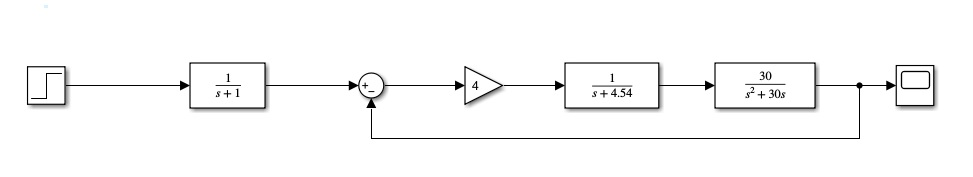
\includegraphics[scale=0.5]{pics/diff.jpg}
    \caption{شمای کلی شبیه سازی در دستگاه معادلات دیفرانسل}
    \label{fig:diff:schema}
\end{figure}
حال برای شبیه سازی در ابتدا بر روی خود مولد
\lr{step}
دو بار کلیک می‌کنیم و
\lr{Final Value}
را برابر 30 قرار می‌دهیم. در نهایت نیز زمان شبیه سازی را برابر 30 قرار می‌دهیم و بر روی دکمه‌ی
\lr{Run}
کلیک می‌کنیم. سپس با دوبار کلیک کردن بر روی
\lr{scope}ای
که قرار داده‌ایم. تنظیمات را می‌توانید در شکل
\ref{fig:diff:settings}
مشاهده کنید.
\begin{figure}[H]
    \centering
    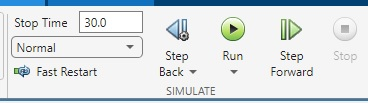
\includegraphics[scale=0.8]{pics/diff_simulate.jpg}
    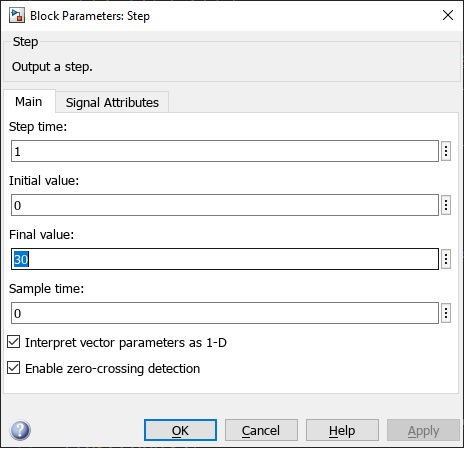
\includegraphics[scale=0.5]{pics/step.jpg}
    \caption{تنظیمات شبیه‌سازی}
    \label{fig:diff:settings}
\end{figure}
همچنین نتیجه‌ی شبیه سازی در شکل
\ref{fig:diff:results}
آمده است.
\begin{figure}[H]
    \centering
    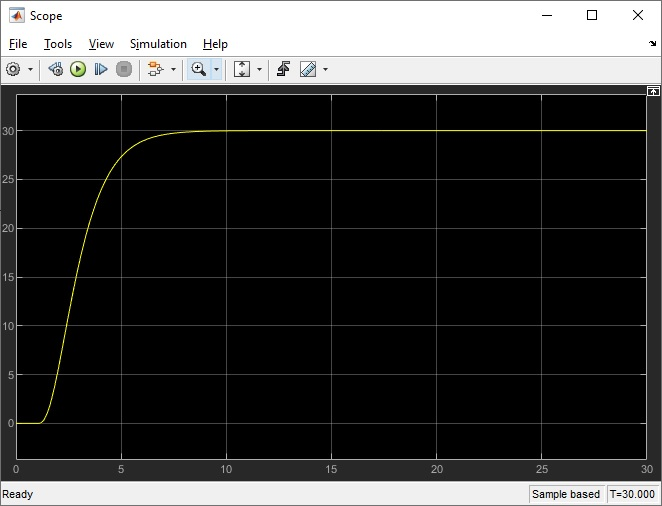
\includegraphics[scale=0.8]{pics/diff_result.jpg}
    \caption{نتیجه شبیه‌سازی در پارادایم معادلات دیفرانسل}
    \label{fig:diff:results}
\end{figure}
\section{شبیه سازی به کمک \lr{State Flow}}
در این قسمت در ابتدا از ساختن یک پروژه‌ی جدید شروع می‌کنیم. سپس مانند دستور کار شمای کلی مدار را
در یک پروژه رسم می‌کنیم.
\begin{figure}[H]
    \centering
    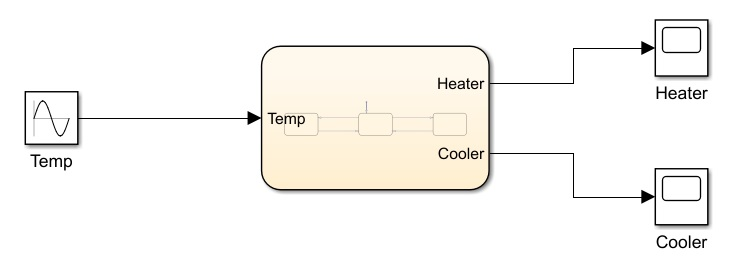
\includegraphics[scale=0.6]{pics/charts_schema1.jpg}
    \caption{شمای کلی مدار در پارادایم \lr{state charts}}
    \label{fig:charts:schema1}
\end{figure}
همچنین در قسمت
\lr{state charts}
نیز مانند شکل داده شده در گزارش کار طراحی حالت‌ها را انجام می‌دهیم. شمای آن در شکل
\ref{fig:charts:schema2}
آمده است.
\begin{figure}[H]
    \centering
    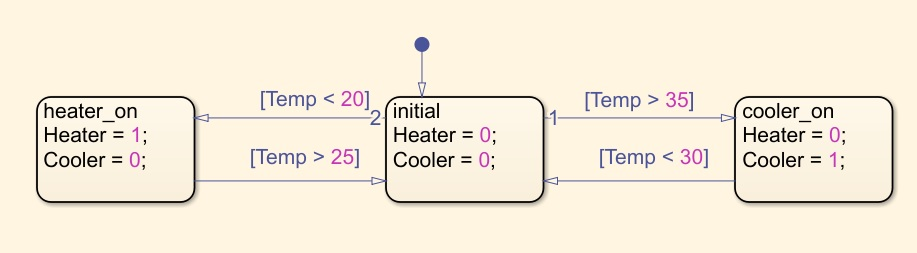
\includegraphics[scale=0.6]{pics/charts_schema2.jpg}
    \caption{شمای کلی حالت‌های مدار در پارادایم \lr{state charts}}
    \label{fig:charts:schema2}
\end{figure}
در نهایت نیز کافی است که تنظیمات موج سینوسی سازنده و زمان شبیه سازی را انجام دهیم. من به صورت شکل
\ref{fig:charts:settings}
این تنظیمات را انجام داده‌ام.
\begin{figure}[H]
    \centering
    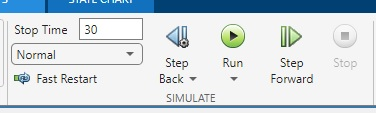
\includegraphics[scale=0.6]{pics/charts_simulate.jpg}
    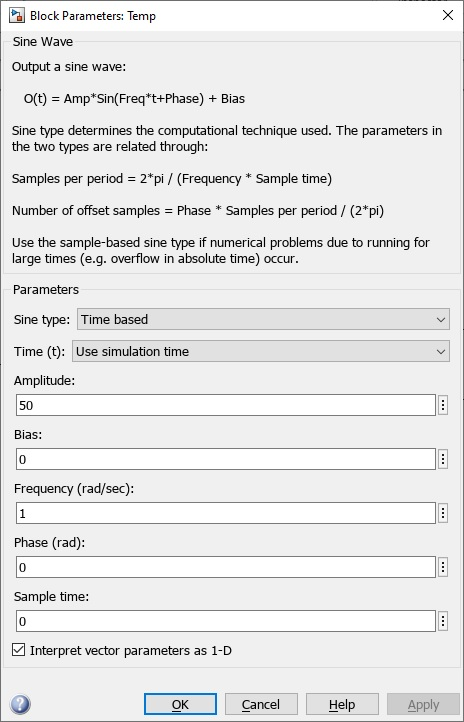
\includegraphics[scale=0.6]{pics/sine.jpg}
    \caption{ تنظیمات شبیه سازی در پارادایم \lr{state charts}}
    \label{fig:charts:settings}
\end{figure}
در نهایت نیز شبیه سازی را اجرا می‌کنیم و نتایج خواسته شده را مشاهده می‌کنیم.
\begin{figure}[H]
    \centering
    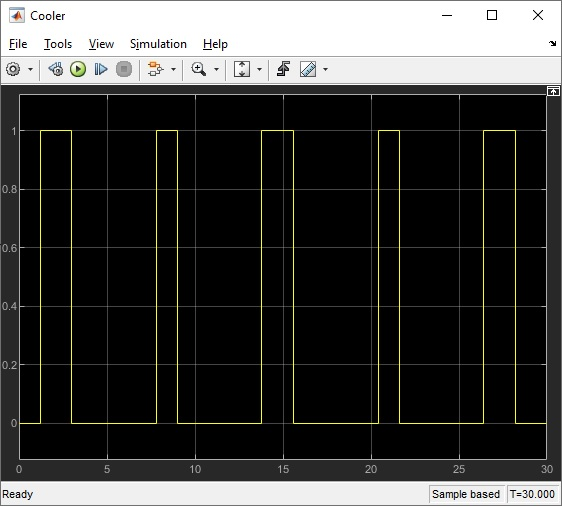
\includegraphics[scale=0.6]{pics/cooler.jpg}
    \caption{خروجی \lr{cooler}}
\end{figure}
\begin{figure}[H]
    \centering
    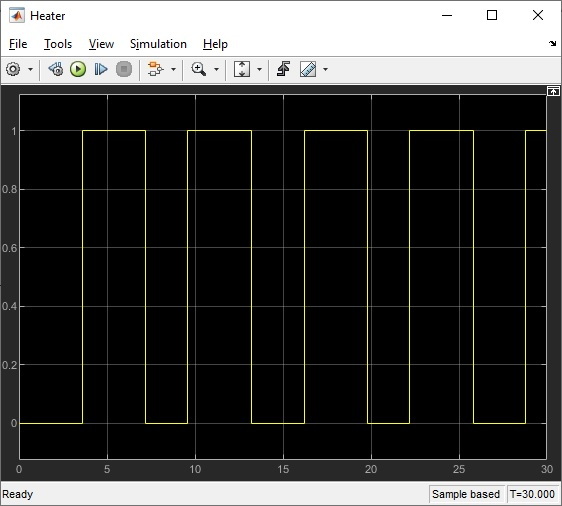
\includegraphics[scale=0.6]{pics/heater.jpg}
    \caption{خروجی \lr{heater}}
\end{figure}
\end{document}
